\documentclass[../main.tex]{subfiles}
\graphicspath{{\subfix{../Images}}}

\begin{document}
\section{Introduction}
\label{sec:introduction}

For the last 15 years, blockchain has been one of the most disruptive fields in academic research. The first blockchain applications made available to the wider public were cryptocurrencies, fully digitalized currencies that could be used to abstract products and services since they had a fiat price associated to it and, therefore, value. But a new way to conduct finances was just the beginning. In parallel with cryptocurrency projects, researchers and enthusiasts begun to experiment with a similar but functionally different token-based concept. Shortly after the release of Bitcoin, the first blockchain cryptocurrency in history, the first Non-Fungible Token project actually was based in the Namecoin blockchain, an offshoot project that sat somewhere between Bitcoin and Ethereum. The Quantum project \cite{Exmundo2023} was started by digital artists Jennifer and Kevin McKoy. After creating the image depicted in Fig. \ref{fig:quantum_nft}, they wanted to be able to sell this artwork in its digital form. The main problem was to find a verifiable way to establish the provenance of that digital piece of art. After collaborating with technology experts, they decided to register the work in the Namecoin blockchain, but using a different approach than the one used to establish ownership of cryptocurrencies, which was by far the main application of the early public blockchains of the 2010s. The ownership relations established by registering the image in the blockchain and "locking" its owner to a single account address at all times prove to be transformative. In some aspects, they simply adapted the ownership mechanics of cryptocurrencies, also known as Fungible Tokens, to another type of token that could be used to represent an actual unique object, which can be digital or physical. Given the contradictory operations of these tokens when compared to the Fungible ones, it was only natural to name these as \textit{Non-Fungible Tokens (NFTs)}.
\par

\begin{figure}[htp]
    \centering
    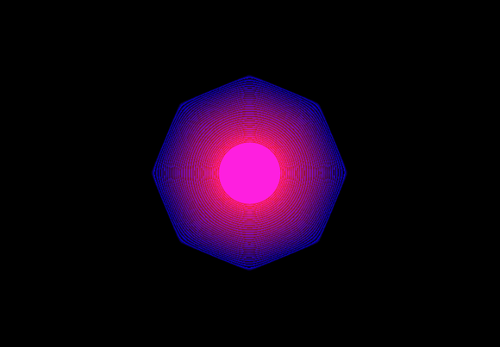
\includegraphics[width=0.9\textwidth]{../Images/02_QuantumNFT.png}
    \caption{Quantum, the first work of art to be encoded into the metadata of an NFT \cite{Exmundo2023}}
    \label{fig:quantum_nft}
\end{figure}
% // TODO: Should this image be set to grayscale for publishing?

Quantum was followed by other, arguably more successful, NFT projects, mostly establishing ownership of digital artworks. Popular projects such as \textit{CryptoPunks} \cite{nftnow2024} and the \textit{Bored Ape Yatch Club (BAYC)}, followed a similar trend as in Quantum and created finite sets of artistic NFTs that were sold directly to users, or even given away to whomever requested them, as it happen during the early days of \textit{CryptoPunks} due to how unusual it was to buy something with crypto. Both these projects are deployed in Ethereum and transactions with these NFTs use Ethers (ETH), Ethereum's native cryptocurrency.
\par
Both projects minted "static" NFTs in which their metadata, which is used to encode an image, either directly in the blockchain (costly) or indirectly by saving the image in a distributed repository and save its url in the NFT metadata instead (cheaper). The \textit{CryptoKitties} NFT project \cite{Dapper2017} followed the previous two but with a slight difference. Each \textit{CryptoKitty} was similar to a \textit{CryptoPunk} in the sense that the image encoded in the NFT was created from an internal parameter of the NFT, and not just some random image file. The characteristics of each \textit{CryptoKitty} were derived from an internal "genome", a 256-bit string from which substrings encoding the token characteristics (eye color, fur color, ear type, tail shape, etc.) were derived. But unlike \textit{CryptoPunks}, \textit{CryptoKitties} could be "bred" to generate new ones with characteristics derived semi-randomly from the parents genome. This dynamic, almost gaming, aspect of \textit{CryptoKitties} proved to be quite attractive to collectors and enthusiast, which translated in a peak of NFT activity in Ethereum that pushed the network to and above its limits \cite{bbc2017}.
\par
The \textit{CryptoKitties} project exposed the limitations of the Ethereum network, particularly regarding scalability. Initially, the team behind the project (initially named \textit{Axiom Zen} but later renamed to \textit{Dapper Labs}) tried to address these problems from withing the Ethereum framework, but with little success. After a while, it became clear that a new blockchain architecture was needed to fully solve the issues encountered and this is how the \textit{Flow} blockchain came to existence.
\par
The approach taken with Flow is quite different than Ethereum from an internal perspective, but for a regular user, interacting with a Flow smart contract or NFT is not much different than with any other NFT. Just like Ethereum introduced \textit{Solidity} as the smart contract programming language for Ethereum contracts, Flow developed \textit{Cadence} with the exact same purpose, albeit with a significant change in how programming principles are approached. The most glaring difference between these two blockchains is how they approach data storage and ownership within the chain. Ethereum stores NFT metadata in a semi-centralised, contract-based fashion, it the sense that the central address is the one where the smart contract that regulates the NFT behavior was deployed, and all storage derives from this point. Flow has a radical approach in this sense, extending the concept of an account from just an address, as it goes in Ethereum, to use this address as a preamble to access a storage area that is unique and individual to each account, i.e., only the owner of the account has access to digital objects stored in the account's storage area. Flow also uses a similar strategy to \textit{gas} to protect and limit the storage space associated to each account, in which the storage space available is proportional to the amount of cryptocurrency staked in that account. Just as Ethereum uses Ether (ETH), \textit{Flow} uses the \textit{FLOW} token as its cryptocurrency used to pay gas fees and to sustain the account's storage area.
\par
These differences, as well as the fact that the Flow blockchain was created precisely to address the limitations of the Ethereum blockchain regarding NFT interoperability, justify this article. In this work we detail how NFTs are implemented in each of the blockchains considered - Flow and Ethereum - in order to provide an objective comparison between them, as well as infer on how well the Ethereum limitations identified by the \textit{CryptoKitties} project were improved in Flow.
\par
The rest of this article is structured as follows: Section \ref{sec:related_works} provides an overview of publications relevant to our work in this article. In Section \ref{sec:background} we provide an introduction to concepts that are key in this work that some readers might not be as familiar as needed to fully understand this publication. Section \ref{sec:solidity_ethereum_nft_implementation} details the construction and deployment of an \textit{ERC-721} compliant NFT Solidity smart contract in the Ethereum network, while Section \ref{sec:cadence_flow_nft_implementation} repeats the same process but for the Flow blockchain, which uses Cadence as the programming language to construct smart contracts. Section \ref{sec:results_and_comparison} provides a summary of our findings, as well as a comparison between the two implementations. This article concludes with Section \ref{sec:conclusion}.
\end{document}

% // TODO: Elaborate on how NFTs can be used to represent ownership of physical, real objects, not just digital ones.

% // TODO: Dynamic NFTs, or NFT 2.0, according to Barbara and Andrea's article, are very important for the downstream application but are not considered in this particular case. Check if it is a good idea to mention this at this point or later on.

% // TODO: Move a lot of the stuff here to the Background.
% // TODO: The Introduction should be short
% // TODO: The contributions of this paper must happen at the end, after the comparison